% Provenance (never printed): cycle 2 "Explorer les organisations du monde ---
% identifier des paysages" (littoraux, massifs montagneux, campagnes, villes),
% see sources/book1/PROVENANCE.md. Book 1, grade 1, chapter 2.
\chapter{المناظر من حولنا}\label{ch:g1:landscapes-around-us}

صعدت ميا وجدها \omterm{def:g1:landscapes-around-us:landform}{التلة} التي خلف القرية حتى قمتها. وفي الأعلى جلسا على
العشب ليستريحا، وأخذا ينظران. تحتهما تتجمع سطوح القرية الحمراء حول
الكنيسة. \omterm{def:g1:landscapes-around-us:water}{ونهر} يتعرج بين حقول خضراء وصفراء ويمر تحت جسر. وعلى \omterm{def:g1:landscapes-around-us:landform}{التلة}
المجاورة غابة داكنة. وبعيدًا، بعيدًا جدًا، في آخر اليابسة، خط رفيع
أزرق.

يقول جدها: «ذلك هو البحر.»

كل ما تراه ميا من قمة \omterm{def:g1:landscapes-around-us:landform}{التلة}، قريبًا كان أو بعيدًا، هو
\omterm{def:g1:landscapes-around-us:landscape}{منظر}.

\begin{omfigure}
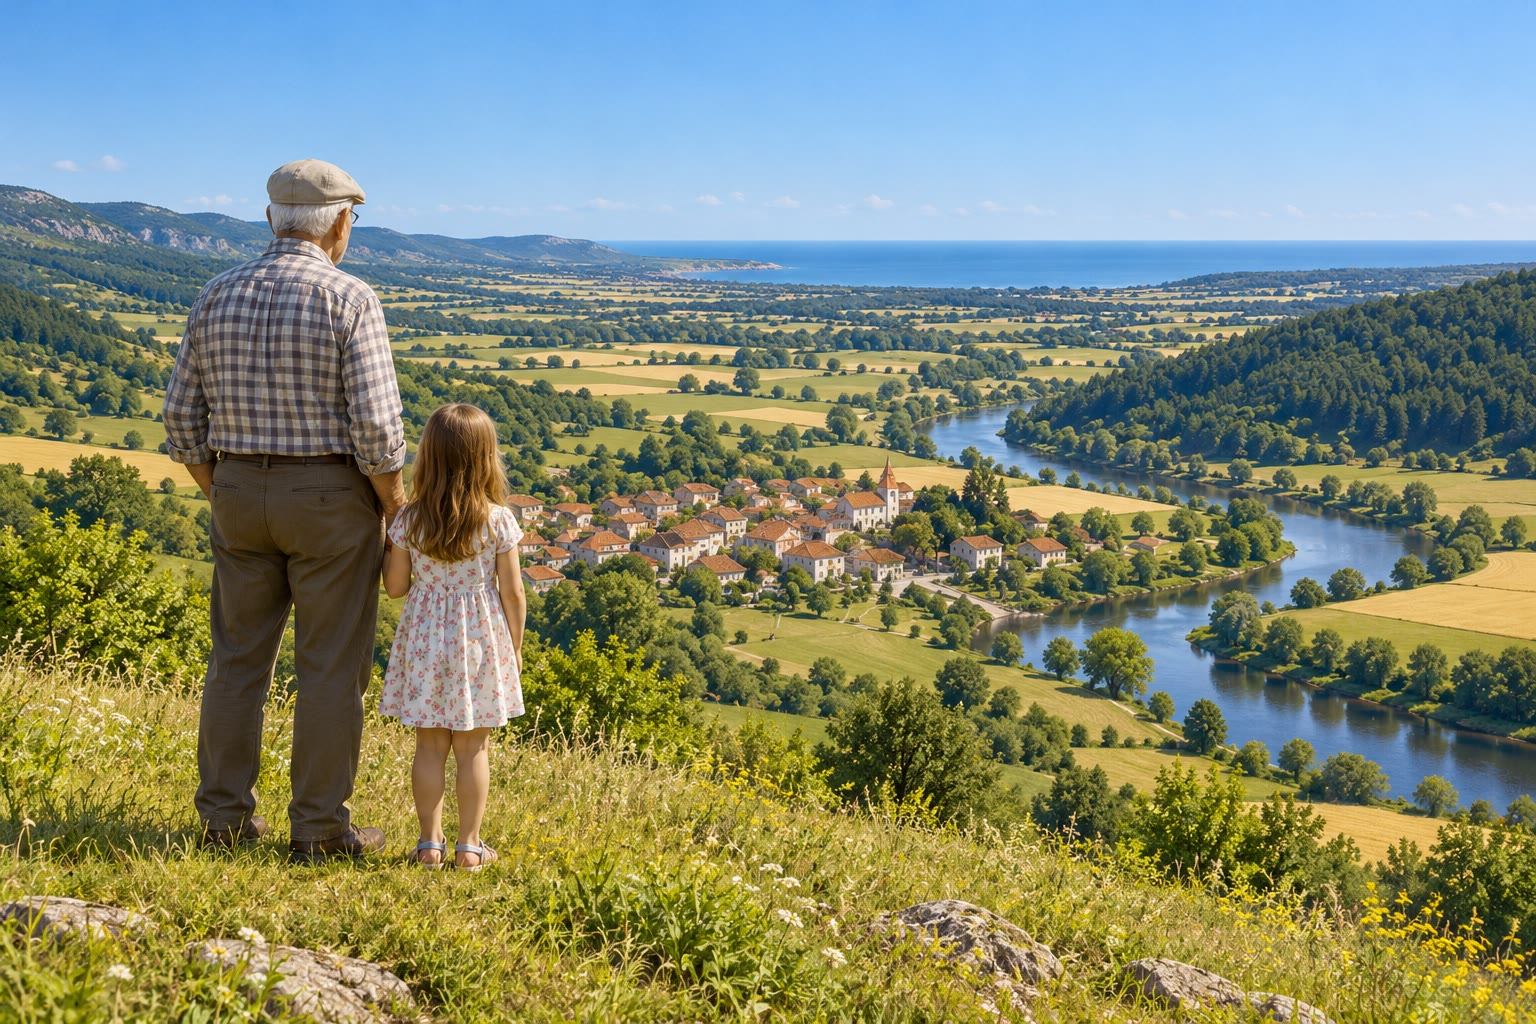
\includegraphics[width=0.72\linewidth]{images/book1/ai/g1-hilltop-view.jpg}

{\small من قمة \omterm{def:g1:landscapes-around-us:landform}{تلة} نرى منظرًا كاملًا.}
\end{omfigure}

\section{ما المنظر؟}

\begin{definition}[المنظر]\label{def:g1:landscapes-around-us:landscape}
\emph{المنظر}\index{منظر} هو كل ما نراه من الأرض بنظرة واحدة، من المكان
الذي نقف فيه حتى الأفق البعيد: شكل الأرض، والماء، والنباتات، والأشياء
التي بناها الناس.
\end{definition}

في \omterm{def:g1:landscapes-around-us:landscape}{المنظر} أجزاء قريبة وأجزاء بعيدة. الجزء الأقرب إلينا يكون في أسفل ما
نراه؛ يبدو كبيرًا ونرى تفاصيله. والجزء البعيد يكون في الأعلى، قرب
السماء؛ يبدو صغيرًا باهتًا.

\begin{omfigure}
\begin{tikzpicture}[x=1cm, y=1cm]
  \fill[ocBlue!12] (0,0) rectangle (10,5);
  % background: far hills
  \fill[black!18] (0,3.0) -- (1.5,3.6) -- (3,3.3) -- (5,3.9) -- (7,3.4) -- (8.5,3.8) -- (10,3.3) -- (10,2.9) -- (0,2.9) -- cycle;
  % middle: hills and fields
  \fill[green!35!omLithAlluv] (0,1.6) -- (2,2.4) -- (4,2.1) -- (6,2.7) -- (8,2.2) -- (10,2.5) -- (10,1.5) -- (0,1.5) -- cycle;
  \fill[green!25!omLithAlluv] (0,1.5) rectangle (10,2.95);
  \fill[green!35!omLithAlluv] (0,2.95) -- (2,3.1) -- (4,2.95) -- (6,3.25) -- (8,3.0) -- (10,3.1) -- (10,2.9) -- (0,2.9) -- cycle;
  \foreach \x in {5.6,5.9,6.2} \fill[red!55] (\x,2.25) -- ++(0.12,0.15) -- ++(0.12,-0.15) -- cycle;
  \foreach \x in {5.6,5.9,6.2} \fill[white] (\x+0.03,2.1) rectangle ++(0.18,0.15);
  % foreground
  \fill[green!55!black!60] (0,0) rectangle (10,1.5);
  \foreach \x in {0.8,2.1,8.6} {
    \fill[brown!70!black] (\x-0.06,0.4) rectangle (\x+0.06,0.9);
    \fill[green!45!black] (\x,1.15) circle (0.38);
  }
  % band borders and labels
  \draw[white, line width=1pt, dashed] (0,1.5) -- (10,1.5);
  \draw[white, line width=1pt, dashed] (0,2.95) -- (10,2.95);
  \node[font=\small\bfseries, fill=white, fill opacity=0.8, text opacity=1, inner sep=2pt] at (5,0.6) {المستوى الأمامي: قريب، كبير، تفاصيل كثيرة};
  \node[font=\small\bfseries, fill=white, fill opacity=0.8, text opacity=1, inner sep=2pt] at (2.7,2.2) {المستوى الأوسط};
  \node[font=\small\bfseries, fill=white, fill opacity=0.8, text opacity=1, inner sep=2pt] at (5,4.4) {المستوى الخلفي: بعيد، صغير، باهت};
\end{tikzpicture}

{\small \omterm{def:g1:landscapes-around-us:landscape}{منظر} نراه في ثلاثة مستويات: المستوى الأمامي في الأسفل، ثم
المستوى الأوسط، ثم المستوى الخلفي أمام السماء.}
\label{fig:g1:landscapes-around-us:bands}
\end{omfigure}

\section{أشكال الأرض}

ليست الأرض مستوية في كل مكان. ففي بعض الأماكن ترتفع عاليًا نحو السماء؛
وفي أماكن أخرى تنخفض في تجاويف طويلة؛ وفي غيرها تمتد مستوية على مدى
البصر. ونعطي كل شكل اسمًا.

\begin{definition}[أشكال التضاريس]\label{def:g1:landscapes-around-us:landform}
\emph{الشكل التضاريسي}\index{شكل تضاريسي} شكل من أشكال سطح الأرض.
\begin{itemize}
  \item \emph{الجبل}\index{جبل} شكل تضاريسي مرتفع جدًا منحدراته شديدة؛
        وأعلاه يسمى القمة. وأعلى الجبال يغطي الثلج قممها حتى في
        الصيف.
  \item \emph{التلة}\index{تلة} شكل تضاريسي يرتفع عما حوله من الأرض،
        وهو أقل ارتفاعًا من الجبل وأكثر استدارة.
  \item \emph{الوادي}\index{وادٍ} تجويف طويل منخفض بين التلال أو
        الجبال؛ وكثيرًا ما يجري في قاعه \omterm{def:g1:landscapes-around-us:water}{نهر}.
  \item \emph{السهل}\index{سهل} أرض واسعة مستوية منخفضة.
\end{itemize}
\end{definition}

\begin{omfigure}
\begin{tikzpicture}[x=1cm, y=1cm]
  \fill[ocBlue!10] (0,0) rectangle (12.4,4.6);
  % sea
  \fill[omSea] (10.2,0) rectangle (12.4,0.55);
  % land profile: mountains, valley, hill, plain, coast
  \fill[omLithAlluv!80!green] (0,0) -- (0,2.2) -- (0.9,3.3) -- (1.5,3.0) -- (2.2,4.1)
     -- (2.9,2.6) -- (3.6,1.2) -- (3.9,0.9) -- (4.2,1.2) -- (5.0,2.0) -- (5.7,2.2)
     -- (6.4,1.6) -- (7.0,0.95) -- (8.0,0.8) -- (9.5,0.7) -- (10.2,0.6) -- (10.4,0.55)
     -- (10.4,0) -- cycle;
  \draw[black!60, line width=0.6pt] (0,2.2) -- (0.9,3.3) -- (1.5,3.0) -- (2.2,4.1)
     -- (2.9,2.6) -- (3.6,1.2) -- (3.9,0.9) -- (4.2,1.2) -- (5.0,2.0) -- (5.7,2.2)
     -- (6.4,1.6) -- (7.0,0.95) -- (8.0,0.8) -- (9.5,0.7) -- (10.2,0.6) -- (10.4,0.55);
  % snow caps
  \fill[white, draw=black!50, line width=0.3pt] (1.95,3.72) -- (2.2,4.1) -- (2.45,3.72) -- (2.3,3.78) -- (2.2,3.68) -- (2.08,3.78) -- cycle;
  \fill[white, draw=black!50, line width=0.3pt] (0.72,3.08) -- (0.9,3.3) -- (1.05,3.15) -- (0.9,3.12) -- cycle;
  % river in the valley
  \fill[omSea!90!black] (3.75,0.92) rectangle (4.05,0.98);
  % lake on the plain
  \fill[omSea] (7.6,0.82) ellipse (0.5 and 0.07);
  % village on the plain
  \foreach \x in {8.6,8.85,9.1} {
    \fill[white, draw=black!50, line width=0.3pt] (\x,0.74) rectangle ++(0.18,0.16);
    \fill[red!60] (\x-0.02,0.9) -- ++(0.11,0.12) -- ++(0.11,-0.12) -- cycle;
  }
  % labels
  \node[font=\small, above] at (2.2,4.12) {جبل};
  \node[font=\small, above] at (5.6,2.25) {تلة};
  \node[font=\small] at (3.9,1.85) {وادٍ};
  \node[font=\small, above] at (8.2,1.5) {سهل};
  \draw[black!60, thin] (8.2,1.5) -- (8.2,0.85);
  \node[font=\small, align=center] at (11.3,1.4) {بحر};
  \node[font=\scriptsize, below=2pt, fill=white, fill opacity=0.8, text opacity=1, inner sep=1pt] at (7.6,0.35) {بحيرة};
  \draw[black!60, thin] (7.6,0.45) -- (7.6,0.78);
  \node[font=\scriptsize, below=2pt, fill=white, fill opacity=0.8, text opacity=1, inner sep=1pt] at (10.3,0.35) {ساحل};
  \node[font=\scriptsize, fill=white, fill opacity=0.8, text opacity=1, inner sep=1pt] at (3.9,0.2) {نهر};
  \draw[black!60, thin] (3.9,0.32) -- (3.9,0.88);
\end{tikzpicture}

{\small أشكال الأرض، من \omterm{def:g1:landscapes-around-us:landform}{الجبال} حتى البحر، نراها من الجانب (رُسمت
الارتفاعات أعلى بكثير مما هي في الحقيقة).}
\label{fig:g1:landscapes-around-us:profile}
\end{omfigure}

\begin{omfigure}
\begin{minipage}[b]{0.49\linewidth}\centering
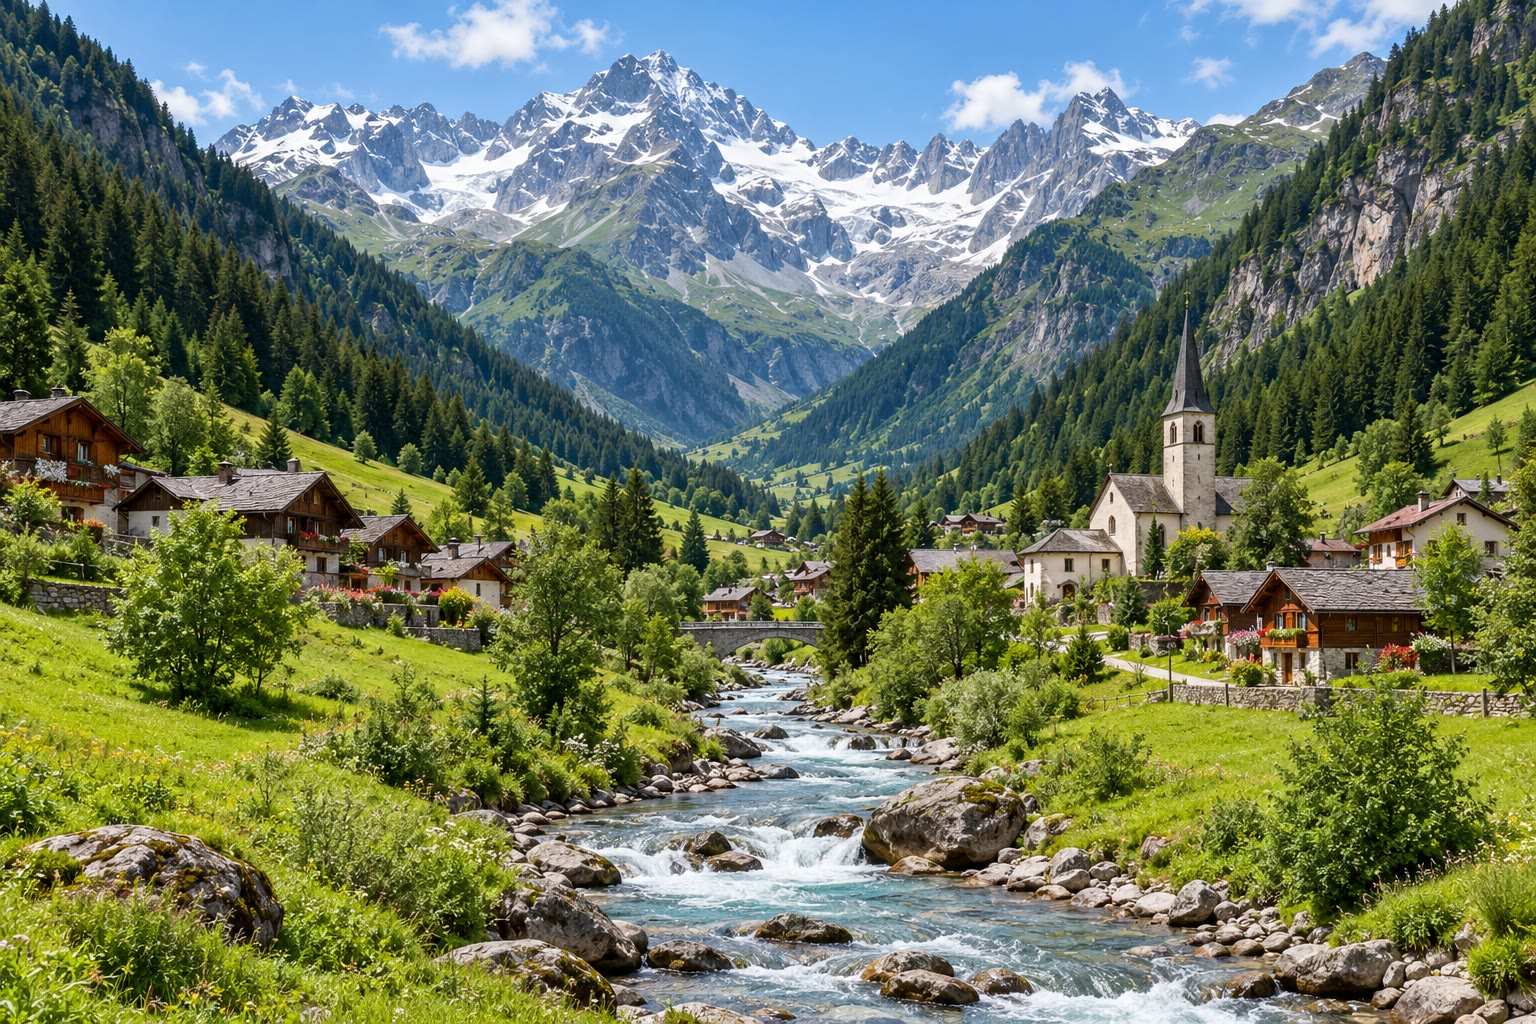
\includegraphics[width=\linewidth]{images/book1/ai/g1-mountain-village.jpg}

{\small \omterm{def:g1:landscapes-around-us:landform}{جبال}، وقرية في واديها.}
\end{minipage}\hfill
\begin{minipage}[b]{0.49\linewidth}\centering
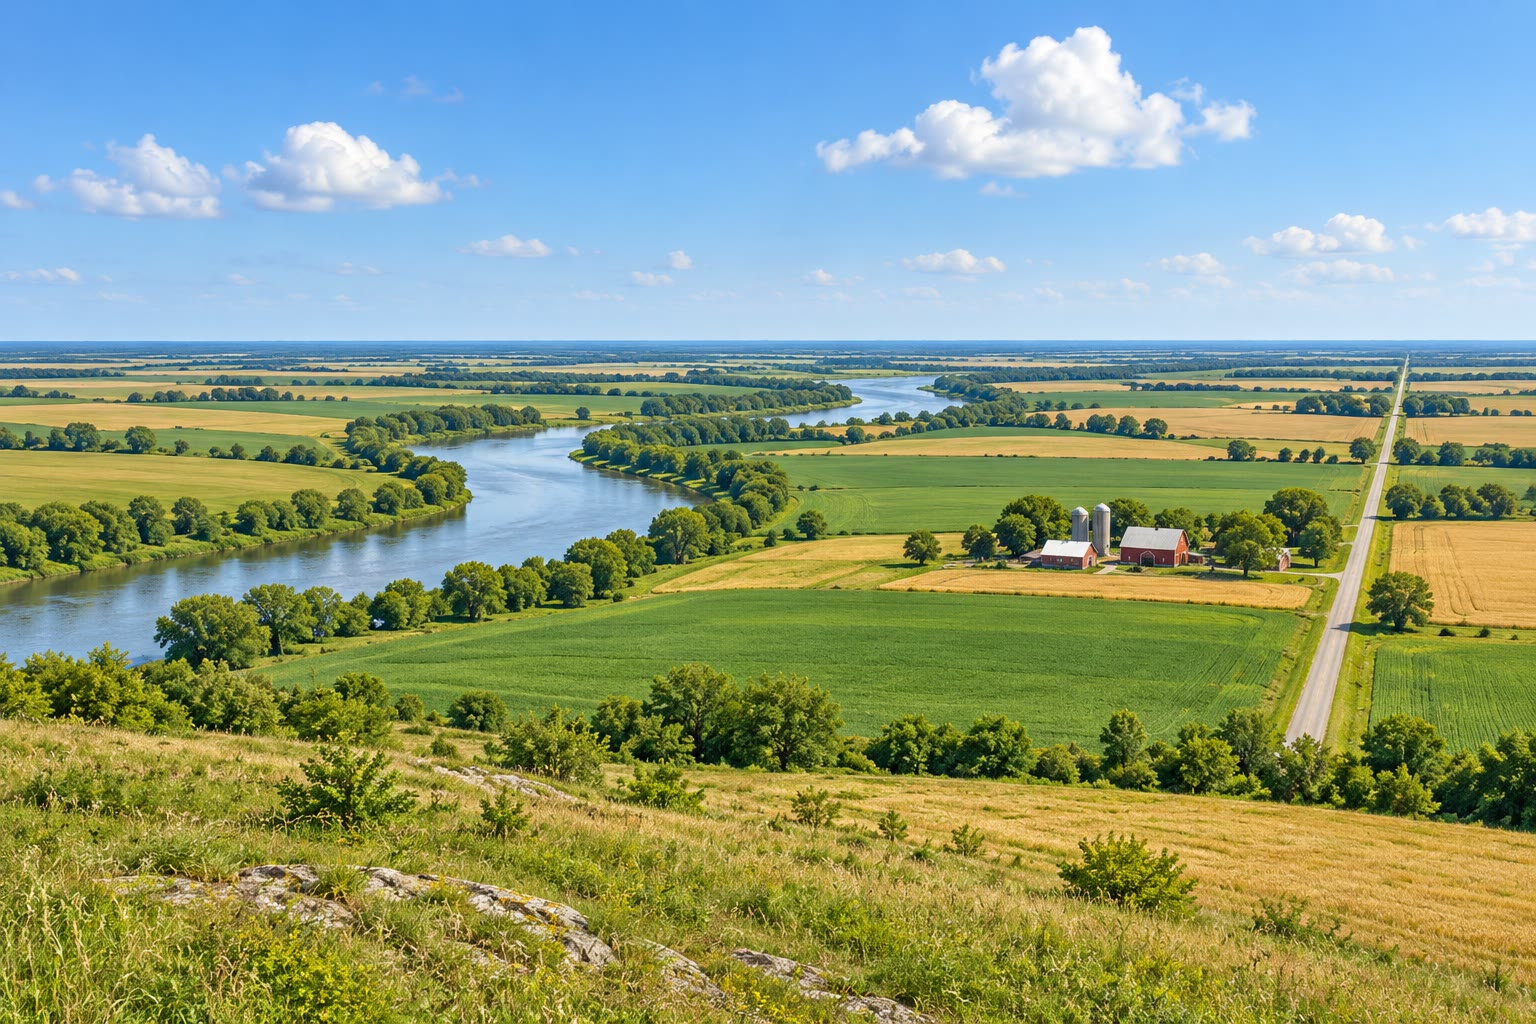
\includegraphics[width=\linewidth]{images/book1/ai/g1-plain-river.jpg}

{\small \omterm{def:g1:landscapes-around-us:landform}{سهل} فيه \omterm{def:g1:landscapes-around-us:water}{نهر} وحقول.}
\end{minipage}
\end{omfigure}

\begin{example}[جبل أم تلة؟]\label{ex:g1:landscapes-around-us:mountain-hill}
لا يوجد ارتفاع محدد تصبح عنده \omterm{def:g1:landscapes-around-us:landform}{التلة} جبلًا. ننظر إلى الشكل: \omterm{def:g1:landscapes-around-us:landform}{الجبل} عالٍ
شديد الانحدار، صخري في الغالب، وعلى قمته ثلج أحيانًا؛ \omterm{def:g1:landscapes-around-us:landform}{والتلة} أقل
ارتفاعًا وأكثر استدارة، يغطيها العشب أو الحقول أو الأشجار في الغالب،
ونستطيع أن نمشي إلى قمتها في وقت قصير.
\end{example}

\section{الماء في المنظر}

الماء جزء من أكثر المناظر. إنه ينحدر من \omterm{def:g1:landscapes-around-us:landform}{التلال} \omterm{def:g1:landscapes-around-us:landform}{والجبال}، ويتجمع في
التجاويف، ويصل إلى البحر.

\begin{definition}[الماء في المنظر]\label{def:g1:landscapes-around-us:water}
\emph{النهر}\index{نهر} ماء يجري طوال الوقت في مجرى طويل، من الأرض
المرتفعة نزولًا إلى بحيرة أو إلى البحر. و\emph{البحيرة}\index{بحيرة}
مساحة كبيرة من الماء تحيط بها اليابسة. و\emph{الساحل}\index{ساحل} هو
المكان الذي تلتقي فيه اليابسة بالبحر.
\end{definition}

\begin{omfigure}
\begin{minipage}[b]{0.49\linewidth}\centering
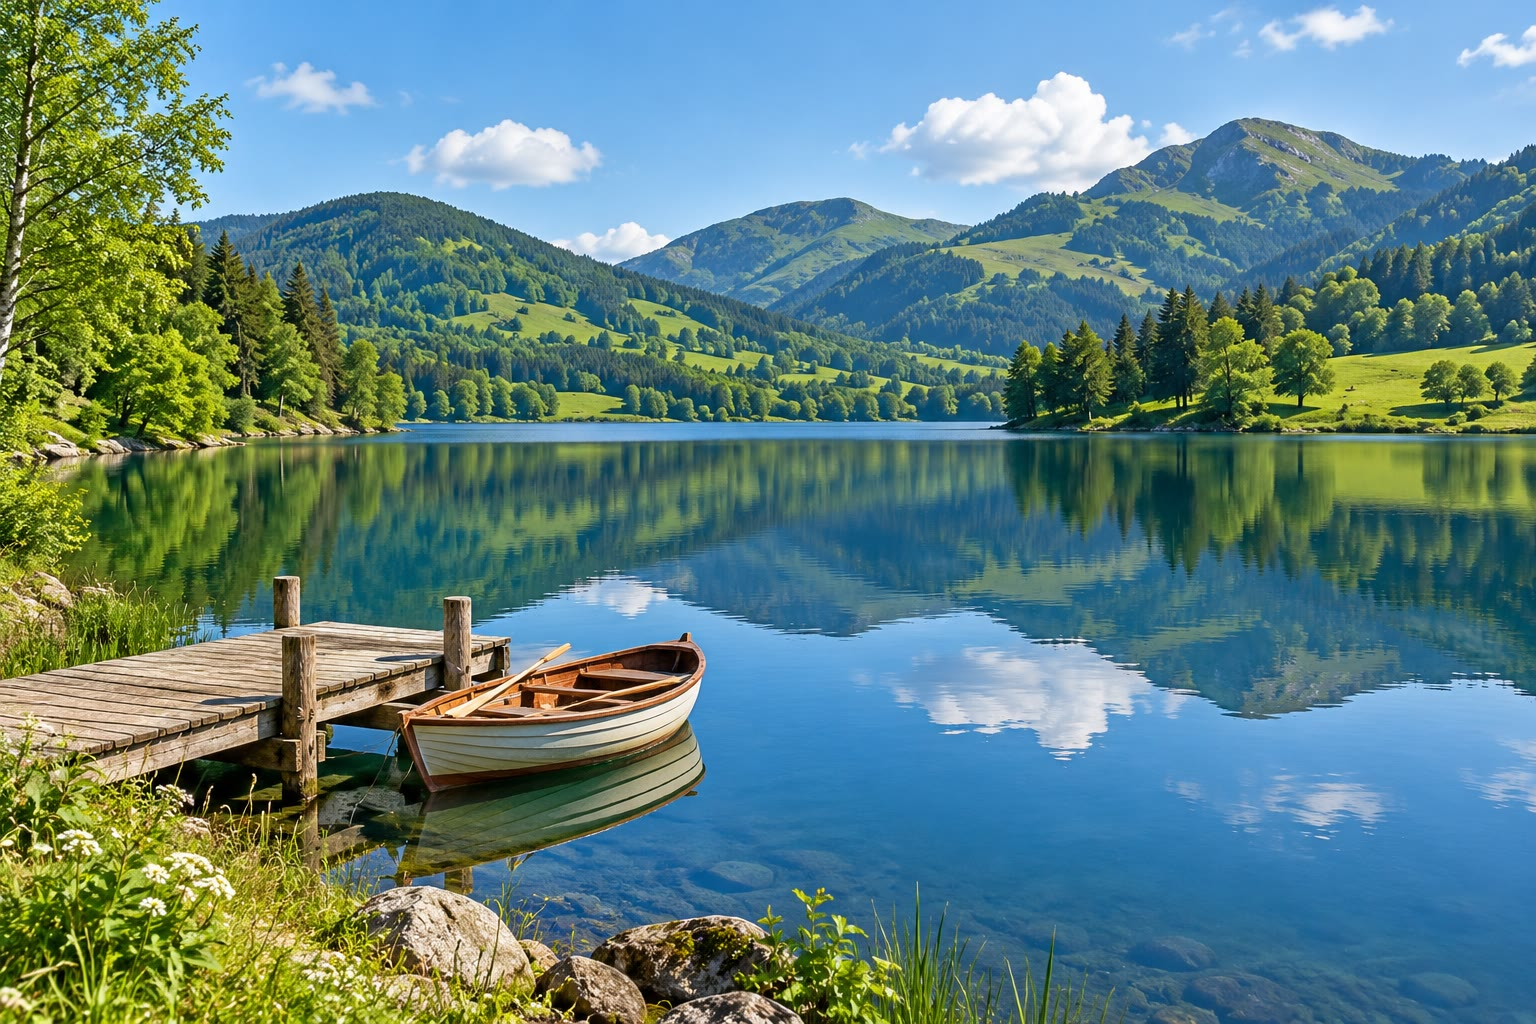
\includegraphics[width=\linewidth]{images/book1/ai/g1-lake-hills.jpg}

{\small \omterm{def:g1:landscapes-around-us:water}{بحيرة} بين \omterm{def:g1:landscapes-around-us:landform}{التلال}.}
\end{minipage}\hfill
\begin{minipage}[b]{0.49\linewidth}\centering
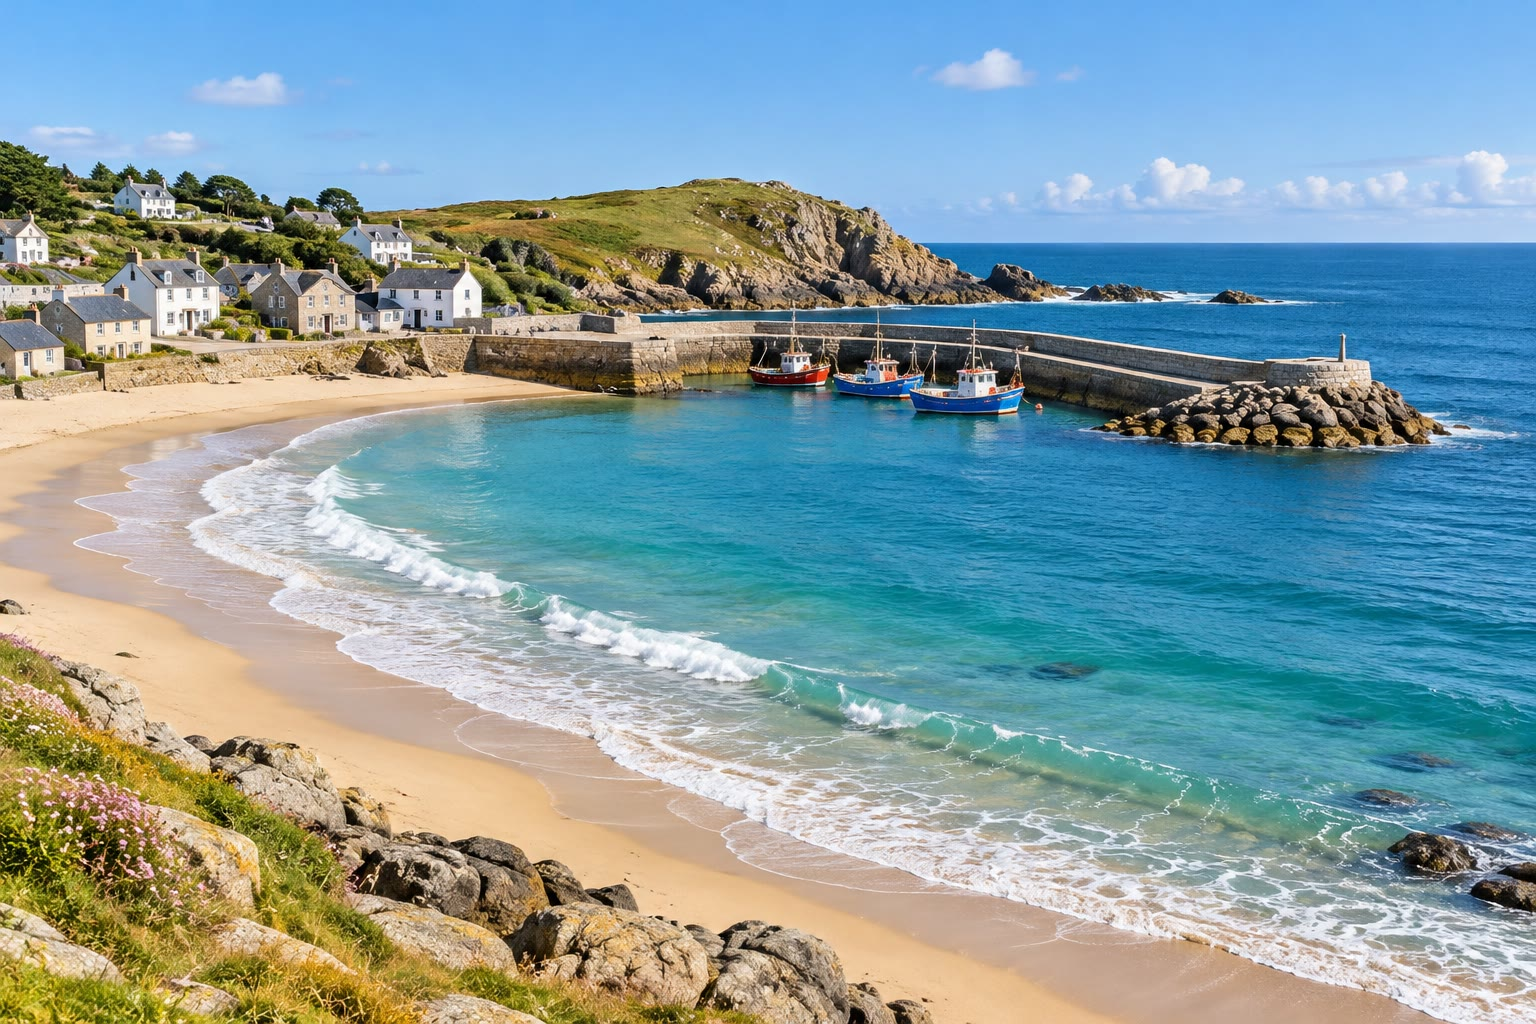
\includegraphics[width=\linewidth]{images/book1/ai/g1-coast-harbour.jpg}

{\small \omterm{def:g1:landscapes-around-us:water}{ساحل}: شاطئ وصخور وميناء.}
\end{minipage}
\end{omfigure}

\begin{remark}[الماء ينحدر دائمًا]\label{rem:g1:landscapes-around-us:downhill}
يجري \omterm{def:g1:landscapes-around-us:water}{النهر} دائمًا من الأرض المرتفعة إلى الأرض المنخفضة. لذلك تجري
\omterm{def:g1:landscapes-around-us:water}{الأنهار} في قيعان \omterm{def:g1:landscapes-around-us:landform}{الأودية}، ولذلك تصل في النهاية إلى \omterm{def:g1:landscapes-around-us:water}{بحيرة} أو إلى البحر،
وهما أخفض من الأرض المحيطة بهما.
\end{remark}

\section{عناصر طبيعية وعناصر من صنع الإنسان}

بعض أجزاء \omterm{def:g1:landscapes-around-us:landscape}{المنظر} كانت موجودة قبل أن يأتي الناس: \omterm{def:g1:landscapes-around-us:landform}{الجبال} \omterm{def:g1:landscapes-around-us:water}{والأنهار}
والغابات. وأجزاء أخرى صنعها الناس: البيوت والطرق والجسور
والحقول.

\begin{definition}[العناصر الطبيعية والعناصر من صنع الإنسان]\label{def:g1:landscapes-around-us:natural-built}
\emph{العنصر الطبيعي}\index{عنصر طبيعي} في \omterm{def:g1:landscapes-around-us:landscape}{المنظر} جزء لم يصنعه الناس:
\omterm{def:g1:landscapes-around-us:landform}{جبل} أو \omterm{def:g1:landscapes-around-us:water}{نهر} أو \omterm{def:g1:landscapes-around-us:water}{بحيرة} أو غابة أو شاطئ.
و\emph{العنصر من صنع الإنسان}\index{عنصر من صنع الإنسان} جزء صنعه الناس
أو شكّلوه: بيت أو طريق أو جسر أو ميناء أو حقل أو حديقة.
\end{definition}

\begin{omfigure}
\begin{tikzpicture}[x=1cm, y=1cm]
  \node[draw=omDef!80!black, fill=omDef!10, rounded corners, text width=5.2cm,
        align=left, minimum height=3.2cm, anchor=north] (n) at (0,0)
    {\textbf{طبيعي}\\[2pt] جبل\\ تلة\\ وادٍ\\ نهر\\ بحيرة\\ غابة\\ شاطئ};
  \node[draw=omMeth!80!black, fill=omMeth!10, rounded corners, text width=5.2cm,
        align=left, minimum height=3.2cm, anchor=north] (b) at (6,0)
    {\textbf{من صنع الإنسان}\\[2pt] بيت\\ كنيسة\\ طريق\\ جسر\\ ميناء\\ حقل\\ حديقة};
\end{tikzpicture}

{\small فرز أجزاء \omterm{def:g1:landscapes-around-us:landscape}{منظر} ميا. الحقل من صنع الإنسان: فالناس أزالوا ما على
الأرض وزرعوها.}
\label{fig:g1:landscapes-around-us:sort}
\end{omfigure}

\section{المناظر تتغير}

لا يبقى \omterm{def:g1:landscapes-around-us:landscape}{المنظر} على حاله إلى الأبد. بعض التغيرات سريع، وبعضها بطيء جدًا
حتى إن أحدًا لا يراه في حياته كلها.
\begin{itemize}
  \item \textbf{مع الفصول:} الحقول بنية بعد الحرث، وخضراء في الربيع،
        وذهبية قبل الحصاد؛ والأشجار تفقد أوراقها في الخريف؛ وقد يغطي
        الثلج كل شيء في الشتاء.
  \item \textbf{بسبب الناس:} تكبر القرية فتصير مدينة؛ وتُقطع غابة لتصنع
        حقول؛ ويعبر طريق جديد وجسر \omterm{def:g1:landscapes-around-us:landform}{الوادي}.
  \item \textbf{بسبب الماء \omterm{def:g1:watching-the-weather:weather}{والطقس}:} بعد عاصفة كبيرة قد يخرج \omterm{def:g1:landscapes-around-us:water}{نهر} من
        مجراه ويغطي الحقول بضعة أيام؛ وعلى \omterm{def:g1:landscapes-around-us:water}{الساحل} تبري الأمواج الصخور
        ببطء.
\end{itemize}

\begin{omfigure}
\begin{tikzpicture}[x=1cm, y=1cm]
  \foreach \k/\t in {0/قديمًا, 1/اليوم} {
  \begin{scope}[shift={(\k*6.4,0)}]
    \fill[ocBlue!8] (0,0) rectangle (5.8,3.4);
    \fill[green!30!omLithAlluv] (0,0) rectangle (5.8,1.9);
    % river
    \fill[omSea] (0,0.55) .. controls (1.5,0.9) and (2.5,0.2) .. (5.8,0.6)
       -- (5.8,0.85) .. controls (2.5,0.45) and (1.5,1.15) .. (0,0.8) -- cycle;
    % hill
    \fill[green!45!black!55] (2.8,1.9) .. controls (3.8,3.1) and (4.8,3.1) .. (5.8,2.2) -- (5.8,1.9) -- cycle;
    \ifnum\k=0
      % forest everywhere, a few houses
      \foreach \x in {0.4,0.9,1.4,1.9,2.4,4.3,4.8,5.3}
        \fill[green!40!black] (\x,1.45) circle (0.22);
      \foreach \x in {3.4,3.75} {
        \fill[white, draw=black!50, line width=0.3pt] (\x,1.15) rectangle ++(0.24,0.2);
        \fill[red!60] (\x-0.03,1.35) -- ++(0.15,0.14) -- ++(0.15,-0.14) -- cycle; }
    \else
      % fields, many houses, a road and a bridge
      \foreach \x/\c in {0.1/yellow!60, 1.3/green!55, 4.5/yellow!45}
        \fill[\c] (\x,1.05) rectangle ++(1.1,0.5);
      \fill[black!35] (2.65,0) rectangle (2.95,1.9);
      \fill[black!55] (2.55,0.5) rectangle (3.05,0.9);
      \foreach \x in {3.2,3.55,3.9} \foreach \y in {1.1,1.45} {
        \fill[white, draw=black!50, line width=0.3pt] (\x,\y) rectangle ++(0.24,0.2);
        \fill[red!60] (\x-0.03,\y+0.2) -- ++(0.15,0.14) -- ++(0.15,-0.14) -- cycle; }
      \foreach \x in {4.6,5.2} \fill[green!40!black] (\x,2.35) circle (0.2);
    \fi
    \node[font=\small\bfseries] at (2.9,-0.3) {\t};
  \end{scope}}
\end{tikzpicture}

{\small \omterm{def:g1:landscapes-around-us:landform}{الوادي} نفسه قديمًا واليوم. \omterm{def:g1:landscapes-around-us:landform}{التلة} \omterm{def:g1:landscapes-around-us:water}{والنهر} لم يتحركا؛ والناس قطعوا
معظم الغابة، وصنعوا حقولًا، وبنوا بيوتًا أكثر وطريقًا
وجسرًا.}
\label{fig:g1:landscapes-around-us:change}
\end{omfigure}

\begin{example}[المدينة والريف]\label{ex:g1:landscapes-around-us:town}
في المدينة، كل ما نراه تقريبًا بناه الناس: شوارع وبيوت ومتاجر وجسور
وحدائق. وفي الريف نرى في الغالب حقولًا وأحراجًا ومروجًا، مع بعض
المزارع والقرى. وكلاهما \omterm{def:g1:landscapes-around-us:landscape}{منظر}. وحتى في وسط مدينة كبيرة تبقى أشكال الأرض
موجودة: \omterm{def:g1:landscapes-around-us:water}{نهر} يعبر المدينة، وبعض الشوارع تصعد
\omterm{def:g1:landscapes-around-us:landform}{تلة}.
\end{example}

\section{وصف المنظر}

\begin{method}[وصف المنظر في أربع خطوات]\label{met:g1:landscapes-around-us:describe}
لوصف \omterm{def:g1:landscapes-around-us:landscape}{منظر}، من قمة \omterm{def:g1:landscapes-around-us:landform}{تلة} أو من صورة:
\begin{enumerate}
  \item \textbf{قسّمه إلى ثلاثة مستويات:} المستوى الأمامي والمستوى الأوسط
        والمستوى الخلفي.
  \item \textbf{سمِّ أشكال الأرض:} \omterm{def:g1:landscapes-around-us:landform}{جبال}، \omterm{def:g1:landscapes-around-us:landform}{تلال}، \omterm{def:g1:landscapes-around-us:landform}{أودية}،
        \omterm{def:g1:landscapes-around-us:landform}{سهول}.
  \item \textbf{ابحث عن الماء:} \omterm{def:g1:landscapes-around-us:water}{نهر}، \omterm{def:g1:landscapes-around-us:water}{بحيرة}، البحر وساحله.
  \item \textbf{ابحث عما بناه الناس:} بيوت، طرق، جسور،
        حقول.
\end{enumerate}
\end{method}

\begin{example}[منظر ميا]\label{ex:g1:landscapes-around-us:mia}
في المستوى الأمامي: العشب في قمة \omterm{def:g1:landscapes-around-us:landform}{التلة}. وفي المستوى الأوسط: \omterm{def:g1:landscapes-around-us:landform}{وادٍ} فيه \omterm{def:g1:landscapes-around-us:water}{نهر}
وجسر وقرية، وحولها حقول، وغابة على \omterm{def:g1:landscapes-around-us:landform}{التلة} المجاورة. وفي المستوى الخلفي:
\omterm{def:g1:landscapes-around-us:landform}{سهل}، وفي آخر اليابسة \omterm{def:g1:landscapes-around-us:water}{الساحل} والبحر. العناصر الطبيعية: \omterm{def:g1:landscapes-around-us:landform}{التلال} \omterm{def:g1:landscapes-around-us:landform}{والوادي}
\omterm{def:g1:landscapes-around-us:water}{والنهر} والغابة والبحر. والعناصر من صنع الإنسان: القرية والكنيسة والجسر
والحقول.
\end{example}

\section{تمارين}

\begin{exercise}[$\star$]\label{exo:g1:landscapes-around-us:1}
سمِّ أشكال الأرض الأربعة التي تعلمتها في هذا الفصل.
\end{exercise}

\begin{exercise}[$\star$]\label{exo:g1:landscapes-around-us:2}
أيهما أعلى وأشد انحدارًا: \omterm{def:g1:landscapes-around-us:landform}{التلة} أم \omterm{def:g1:landscapes-around-us:landform}{الجبل}؟
\end{exercise}

\begin{exercise}[$\star$]\label{exo:g1:landscapes-around-us:3}
طبيعي أم من صنع الإنسان؟ \omterm{def:g1:landscapes-around-us:water}{نهر}؛ طريق؛ غابة؛ جسر؛ شاطئ؛ بيت.
\end{exercise}

\begin{exercise}[$\star$]\label{exo:g1:landscapes-around-us:4}
أين \omterm{def:g1:landscapes-around-us:water}{الساحل}: حيث تلتقي اليابسة \omterm{def:g1:landscapes-around-us:water}{بنهر}، أم حيث تلتقي اليابسة
بالبحر؟
\end{exercise}

\begin{exercise}[$\star$]\label{exo:g1:landscapes-around-us:5}
انظر إلى صورة \omterm{def:g1:landscapes-around-us:landform}{الجبال} وقريتها. سمِّ عنصرًا طبيعيًا واحدًا وعنصرًا واحدًا
من صنع الإنسان.
\end{exercise}

\begin{exercise}[$\star$]\label{exo:g1:landscapes-around-us:6}
في رسم أشكال الأرض، أي \omterm{def:g1:landscapes-around-us:landform}{شكل تضاريسي} هو الأعلى؟
وأين يجري \omterm{def:g1:landscapes-around-us:water}{النهر}؟
\end{exercise}

\begin{exercise}[$\star\star$]\label{exo:g1:landscapes-around-us:7}
من أين يجري \omterm{def:g1:landscapes-around-us:water}{النهر}، وإلى أين يذهب؟ ولماذا لا يجري أبدًا صاعدًا إلى قمة
\omterm{def:g1:landscapes-around-us:landform}{تلة}؟
\end{exercise}

\begin{exercise}[$\star\star$]\label{exo:g1:landscapes-around-us:8}
في صورة \omterm{def:g1:landscapes-around-us:landscape}{منظر}، تبدو شجرة في أسفل الصورة أكبر من \omterm{def:g1:landscapes-around-us:landform}{تلة} كاملة في أعلاها.
لماذا؟
\end{exercise}

\begin{exercise}[$\star\star$]\label{exo:g1:landscapes-around-us:9}
صف صورة \omterm{def:g1:landscapes-around-us:landform}{السهل} ونهره في ثلاثة مستويات: ماذا يوجد في المستوى الأمامي،
وفي المستوى الأوسط، وفي المستوى الخلفي؟
\end{exercise}

\begin{exercise}[$\star\star$]\label{exo:g1:landscapes-around-us:10}
حقل القمح أخضر أو ذهبي، مثل العشب. لماذا نقول إنه \omterm{def:g1:landscapes-around-us:natural-built}{عنصر من صنع الإنسان}
في \omterm{def:g1:landscapes-around-us:landscape}{المنظر} وليس عنصرًا طبيعيًا؟
\end{exercise}

\begin{exercise}[$\star\star$]\label{exo:g1:landscapes-around-us:11}
انظر إلى رسم \omterm{def:g1:landscapes-around-us:landform}{الوادي} قديمًا واليوم. سمِّ شيئين لم يتغيرا وثلاثة أشياء
أضافها الناس.
\end{exercise}
